      \p
فرض کنید مثلث‌ها در مجموع
$v$
راس و
$e$
ضلع داشته باشند.
$n$
تا از راس‌ها، رئوس
$n$
ضلعی هستندو بقیه درون آن قرار دارند. همچنین
$n$
تا از اضلاع، اضلاع
$n$
ضلعی هستند و هر یک فقط ضلع یک مثلث می‌باشند و بقیه درون
$n$
ضلعی قرار دارند و هر یک ضلع دو مثلث هستند.
\begin{center}
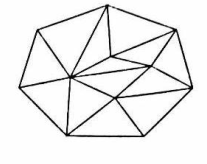
\includegraphics[height=6.5cm]{1.png}
\end{center}
فرض کنید
$S_1$
مجموع زوایا و
$S_2$
مجموع تعداد اضلاع
$m$
مثلث باشد، در این صورت:
$$180m = S_1 = 180(n - 2) + 360(v - n)$$
$$3m = S_2 = n + 2(e - n)$$
از تساوی اول نتیجه می‌گیریم
$m + n = 2v - 2$ 
، لذا
$m + n$
عددی زوج است. همچنین از این دو تساوی نتیجه می‌گیریم:
$$v = \frac{1}{2}(m + n + 2)$$
$$e = \frac{1}{2}(3m + n)$$       